\documentclass[a4paper,11pt]{article}
  
\usepackage{graphicx}
\usepackage{amsmath}
\usepackage{array}
\usepackage{float}
\usepackage{subfigure}
\usepackage{color}
\usepackage{listings}
\usepackage[utf8x]{inputenc}
\usepackage{hyperref}
\usepackage{rotating}

\usepackage{amsfonts,amsmath,amsthm,amssymb}
\usepackage{algorithm}
\usepackage{algpseudocode}

\renewcommand{\algorithmicrequire}{\textbf{Input:}}
\renewcommand{\algorithmicensure}{\textbf{Output:}}

%% --------- Algorithms -------------
\providecommand{\BeginAlgSize}[0]{\begin{scriptsize}}
\providecommand{\EndAlgSize}[0]{\end{scriptsize}}
\providecommand{\ForEach}[1]{\For{\textbf{each} #1}}
\providecommand{\Or}[0]{O}
\providecommand{\A}[0]{\mathbf{\alpha}}
%% --------- End of Algorithms -------------



% Read MRPT version:
\newread\file
\openin\file=../../version_prefix.txt
\read\file to\MRPTVERSION % Reads a line of the file 
\closein\file

% Title Page
\title{User guide for \texttt{libmrpt-srba}: A generic C++ framework for Relative Bundle Adjustment (RBA)}
\author{Jose-Luis Blanco-Claraco \\ joseluisblancoc@gmail.com \\ \texttt{http://www.mrpt.org/} }
\date{MRPT version: \MRPTVERSION \\ Document build: \today }

% C++ listings settings
\lstset{ %
language=C++,                % choose the language of the code
basicstyle=\scriptsize,       % the size of the fonts that are used for the code
numbers=none,                   % where to put the line-numbers
numberstyle=\footnotesize,      % the size of the fonts that are used for the line-numbers
stepnumber=1,                   % the step between two line-numbers. If it is 1 each line will be numbered
numbersep=5pt,                  % how far the line-numbers are from the code
backgroundcolor=\color{white},  % choose the background color. You must add \usepackage{color}
commentstyle=\color{blue},
showspaces=false,               % show spaces adding particular underscores
showstringspaces=false,         % underline spaces within strings
showtabs=false,                 % show tabs within strings adding particular underscores
frame=single,           % adds a frame around the code
tabsize=2,          % sets default tabsize to 2 spaces
captionpos=b,           % sets the caption-position to bottom
breaklines=true,        % sets automatic line breaking
breakatwhitespace=false,    % sets if automatic breaks should only happen at whitespace
escapeinside={\%*}{*)}          % if you want to add a comment within your code
}

\begin{document}
\maketitle


\vfill

\begin{scriptsize}
\begin{center}

\includegraphics[width=3cm]{imgs/by-nc-nd-eu.pdf}
\\
This work is licensed under a Creative Commons Attribution-NonCommercial-NoDerivs 3.0 Unported License.
\end{center}
\end{scriptsize}

\vspace{1cm}

\newpage

\textbf{Revision history:}
\begin{itemize}
 \item Feb 2013: First version. Released along MRPT 1.0.0.
\end{itemize}

\vfill


\begin{small}
In case you want to cite this guide in your academic publications, here is a BibTeX entry: 

\begin{verbatim}
@MISC{libmrpt-srba-guide,
  author = {Jose-Luis Blanco-Claraco},
  title = {{User guide for \texttt{libmrpt-srba}: A generic 
      C++ framework for Relative Bundle Adjustment (RBA)}},
  howpublished = {http://www.mrpt.org/srba},
  year = {2013}
} 
\end{verbatim} 

\end{small}

\vspace{1cm}

\newpage
\tableofcontents
\newpage

\section{Introduction}

Bundle adjustment (BA) is the name given to one solution to visual SLAM based on maximum-likelihood estimation (MLE) 
over the space of map features and camera poses. However, it is by no way limited to visual maps, since the same 
optimization techniques employed in BA are also applicable to maps of pose constraints (graph-SLAM) and to many other 
kind of feature maps, not necessarily involving visual information.

The framework of \emph{Relative Bundle Adjustment (RBA)} was introduced in a series of works by Gabe Sibley and 
colleagues in \cite{sibley2009rba,sibley2009adaptive}. 

\emph{Sparser RBA (SRBA)} is the name of the generic and extensible framework for RBA, implemented in 
the C++ library \texttt{libmrpt-srba}. It features the introduction of 
a \emph{constant-time algorithm} for maintaining problem graphs with arbitrary topologies 
(as presented in \cite{blanco2013srba}), as well as a generic design which allows turning RBA 
into \emph{relative Graph-SLAM} (i.e. networks of relative pose constraints whose solution are also relative poses).

\section{Library installation}

\texttt{libmrpt-srba} is one of the libraries of the Mobile Robot Programming Toolkit (MRPT). 
It is header-only and makes \emph{intensive} use of templates and design patterns for the sake of customization, 
flexibility and extensibility. 

Note however that it depends on other non-header-only libraries\footnote{The link-time dependencies are: \texttt{mrpt-base} 
for geometry, math auxiliary classes, serialization,... and \texttt{mrpt-opengl} for generating 3D representations of 
the RBA problems. Despite its name, the latter library can be built for platforms without any 
functional \texttt{OpenGL} implementation, though it is recommended to always visualize the results for getting a better 
insight of what is going on in your programs. The header-only library \texttt{Eigen} \cite{eigenweb} is also a mandatory dependency, but 
an embedded version is shipped with \texttt{mrpt-base}.}, 
so in practice before using \texttt{libmrpt-srba} in your program you need
both (i) access to headers (\texttt{.h} files) and (ii) binary libraries to link against them. 

In Ubuntu, installing the package \texttt{libmrpt-dev} (version 1.0.0 or newer) is the easiest way to have 
everything ready to start coding your own programs. You can also install \texttt{mrpt-apps} for the application \texttt{srba-slam} 
and a set of sample datasets (see \S\ref{sect:srba_slam_app}).

If your official repository has an older version of the package, use this PPA repository instead:

\begin{lstlisting}
 sudo add-apt-repository ppa:joseluisblancoc/mrpt
 sudo apt-get update
 sudo apt-get install libmrpt-dev mrpt-apps
\end{lstlisting}

Binary packages for Windows are also available online (\href{http://www.mrpt.org/download}{link}).
If you prefer to build MRPT from sources, please visit the official web\footnote{\href{http://www.mrpt.org/}{http://www.mrpt.org/}} 
for detailed instructions.


\section{RBA primer}
\label{sect:rba_primer}

This manual will not explain the mathematical details of how RBA is modeled and solved -- please, refer to cited papers.
Though, it is mandatory to clearly establish which \textbf{entities} define an RBA problem before discussing the library API.

An example such that the one in Fig.~\ref{fig:rba.entities} will help introducing the different elements.
The illustration depicts many elements, some of which are \emph{known} data, others are the problem \emph{unknowns}. 
The goal of RBA is to recover a \emph{maximum-likelihood estimation (MLE)} of those unknowns. Optionally, the covariances and 
cross-covariances between estimated variables can be also evaluated.

\begin{figure}
\centering
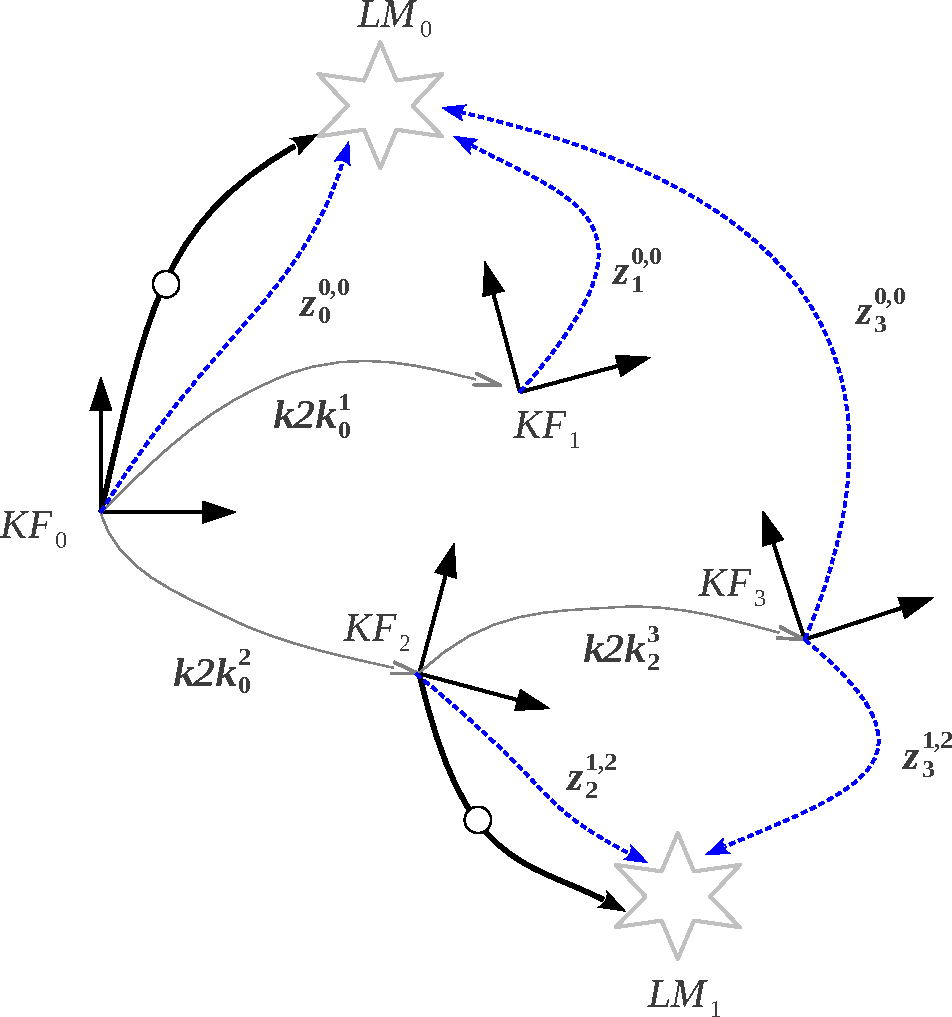
\includegraphics[width=0.7\textwidth]{imgs/srba_toy_problem.pdf} 
\caption{A toy RBA problem.}
\label{fig:rba.entities}
\end{figure}

We find the following entities in \texttt{libmrpt-srba} (refer to Fig.~\ref{fig:rba.entities}):

\begin{itemize}
\item{\textbf{Keyframes}: A keyframe (KF), as each $KF_i$ in the figure, represents the \emph{pose} of the robot (or the 
camera or whatever) at one  particular instant of time. In RBA we will never work with the absolute coordinates of any of 
these KFs. This is completely different than ``common'' Bundle Adjustment, where these poses are the unknowns to 
estimate.
}
\item{\textbf{Keyframe-to-keyframe edges}: An edge $k2k_i^j$ represents the relative pose of $KF_i$ with respect to 
$KF_j$. Notice that ``inverse poses'' (i.e. in the inverse order than one would expect from the edge direction) are 
stored for efficiency\footnote{In RBA we may need to chain sequences of relative poses, and the direction will often 
be from newer KFs towards older KFs, hence if we store inverse poses we save the computational burden of inverting them 
over and over again.}. These edges are always treated as \emph{unknowns} to be estimated from observation data.
They can be parameterized in different ways (see \S\ref{sec:k2k_types}), but in practice it will be enough to work 
with SE(2) or SE(3) poses.
}
\item{\textbf{Landmarks}: A landmark (LM) is any entity which can be observed from different locations. Typically a 2D 
or 3D point in space, but could be a line, segment, plane or any user-defined entity. They are represented in 
the Fig.~\ref{fig:rba.entities} as stars named $LM_i$. The concept of absolute coordinates of a LM 
does not exist in RBA.
}
\item{\textbf{Relative position and "base keyframe" of a LM}: Each LM is associated to exactly one KF, its {base KF}, with 
respect to which the LM has a \emph{relative position}. This relative position can be either ``known'' (``\emph{fixed}'' 
in the C++ API) or ``unknown'', in which case it is also estimated during the problem optimization. There exist several 
possible ways of parameterizing relative positions, as discussed in \S\ref{sec:k2f_types}. These relative positions are 
represented in the figure as thick edges with a middle circle mark.
}
\item{\textbf{Observations}: An observation $z^{i,j}_k$ stands for any piece of sensory data which \emph{is related}, 
somehow, with the position of the $i-th$ LM, whose base KF is $j$, as seen from the observing KF $k$. They are 
depicted as dashed lines in the figure above. Rank-deficient observations, like those from monocular cameras, are 
acceptable but two or more observations may be required before being able to estimate the relative position of the 
observed LM.
}
\end{itemize}

\newpage


\section{Programmer's first steps}
\label{sect:program_first}

The central class in \texttt{libmrpt-srba} is the template \texttt{RbaEngine<>}, which 
adopts a ``policy-based design'' \cite{andrei2001modern}:

\begin{lstlisting}
template <
	class KF2KF_POSE_TYPE,
	class LM_TYPE,
	class OBS_TYPE, 
	class RBA_OPTIONS = RBA_OPTIONS_DEFAULT>
class RbaEngine;
\end{lstlisting}

This means that by setting each of the \emph{template arguments} we literally control the process 
of code generation to address one particular instance of a RBA problem. 
Since all this happens at \emph{compile time}, the compiler produces optimized code for 
the problem at hand (e.g. SSE2 code for multiplying matrices of a particular size), 
avoids code bifurcations, etc.

Due to the combinatorial nature of all the possibilities, 
detailed in \S\ref{sect:rba_configs}--\ref{sect:rba_options}, one template class 
can generate specialized code for dozens of concrete problems. 
The only price to pay is the longer build time associated to any complex C++ program 
that exploits metaprogramming with templates.


\subsection{The simplest program}

The following code illustrates the declaration of an RBA problem for 3D point landmarks, 
with SE(3) relative poses for keyframes and 3D range-bearing observations. 
Only two keyframes are defined, which means that after introducing the second one
there will be only one k2k edge (an unknown), which will be estimated by the least-squares 
optimizer along the relative positions of all landmarks.

\begin{lstlisting}
#include <mrpt/srba.h>

using namespace mrpt::srba;
using namespace std;

typedef RbaEngine<
	kf2kf_poses::SE3,       // Parameterization  KF-to-KF poses
	landmarks::Euclidean3D, // Parameterization of landmark positions    
	observations::RangeBearing_3D // Type of observations
	>
	my_srba_t;

int main(int argc, char**argv)
{
	my_srba_t rba;  //  Create an empty RBA problem
	
	// Define observations of KF #0:
	// ----------------------------------------------
	my_srba_t::new_kf_observations_t  list_obs;
	my_srba_t::new_kf_observation_t   obs_field;
	obs_field.is_fixed = false; // Landmarks have unknown relative 
	                            // positions (i.e. are unknowns )
	obs_field.is_unknown_with_init_val = false; // We don't have 
       // any guess on the initial LM position (will invoke the 
       // inverse sensor model)

	// For each observation:
	for (...) {
		obs_field.obs.feat_id = ...; // The landmark ID
		obs_field.obs.obs_data.range = ...;
		obs_field.obs.obs_data.yaw   = ...;
		obs_field.obs.obs_data.pitch = ...;
		list_obs.push_back( obs_field );
	}

	//  This is the main API entry point: Define KF #0
	my_srba_t::TNewKeyFrameInfo new_kf_info; // Placeholder of out info.
	rba.define_new_keyframe(
		list_obs,      // Input observations for the new KF
		new_kf_info,   // Output info
		true           // Run optimization of the local area
		);

	// Define observations of KF #1:
	// ----------------------------------------------
	list_obs.clear();
	// For each observation:
	for (...) {
		obs_field.obs.feat_id = ...; // The landmark ID
		obs_field.obs.obs_data.range = ...;
		obs_field.obs.obs_data.yaw   = ...;
		obs_field.obs.obs_data.pitch = ...;
		list_obs.push_back( obs_field );
	}

	//  This is the main API entry point: Define KF #1
	rba.define_new_keyframe(
		list_obs,      // Input observations for the new KF
		new_kf_info,   // Output info
		true           // Run optimization of the local area
		);

	cout << "Created KF #" << new_kf_info.kf_id 
	 << " | # kf-to-kf edges created:" <<  
	 new_kf_info.created_edge_ids.size() << endl <<
	 "Optimization error: " << 
	 new_kf_info.optimize_results.total_sqr_error_init << 
	 " -> " << 
	 new_kf_info.optimize_results.total_sqr_error_final << endl;

	// Save RBA graph as Graphviz file:
	rba.save_graph_as_dot("graph.dot", true /* LMs=save */);

	return 0;
}
\end{lstlisting}

\newpage

\subsection{API entry points}

It must be highlighted that, at present, the only API for inserting new KFs 
into the RBA problem is the method \texttt{define\_new\_keyframe()}:

\begin{lstlisting}
template <...> class RbaEngine {
    ...
	void define_new_keyframe(
		const typename traits_t::new_kf_observations_t  & obs,
		TNewKeyFrameInfo  & out_new_kf_info,
		const bool        run_local_optimization = true
		);
    ...
};
\end{lstlisting}

\noindent which accepts as its main input the list of all the observations gathered at this 
new KF. This method \emph{always creates a new KF}, without analyzing whether it was 
too close or too far from the last one. Thus, it is (for now) the user's responsibility 
not to call the method too often, which would create an unnecessarily large amount of KFs with 
the subsequent degradation of the performance. \emph{The constant-time complexity} of the overall 
method assumes that there exists a maximum number of KFs per area --which is perfectly reasonable.

As output, this method provides a structure with:
\begin{itemize}
 \item The ID of the newly-created KF. 
 \item{ The list of all the created KF-to-KF edges. At least one, or more in the case of loop-closures. 
        The way in which edges are created depends on the \emph{edge-creation policy} (see \S\ref{sect:edge.policy}).
        An exception will be raised if no suitable edge is found to connect the new KF to the existing graph.}
 \item The numerical results from the local optimization process: the exact list of unknowns that undergone optimization, 
       the initial and final root mean-squared error (RMSE), etc.
\end{itemize}

Please, refer to the pseudocode description of this method 
in \S\ref{sect:code:define_new_keyframe} for a better insight of 
what happens inside.


\newpage

\subsection{Tutorials}

More complete versions of the program above, including sample datasets and rendering of the optimization result 
as OpenGL scenes are shipped with MRPT\footnote{See the directory \texttt{[MRPT]/samples/srba-examples/srba-tutorials/}, 
or \href{http://mrpt.googlecode.com/svn/trunk/samples/srba-examples/srba-tutorials/}{browse online}.}.
Screenshots are shown in Figs.~\ref{fig:screenshot.tutorial1}--\ref{fig:screenshot.tutorial2}.

\begin{figure}[h]
\centering
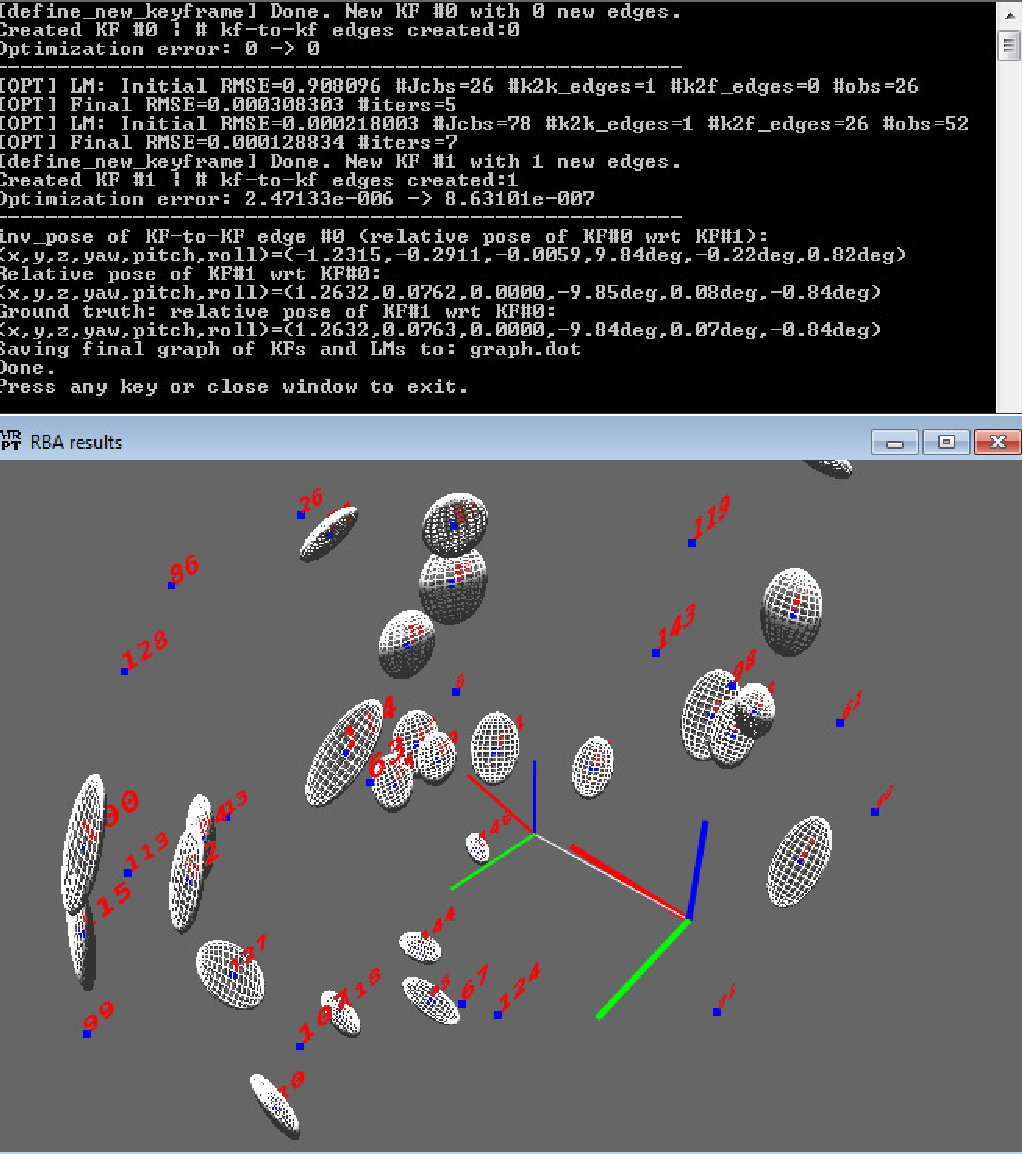
\includegraphics[width=0.9\textwidth]{imgs/screenshot_tutorial_range-bearing-3D.pdf} 
\caption{Screenshot for \texttt{tutorial-srba-range-bearing-se3.cpp}.}
\label{fig:screenshot.tutorial1}
\end{figure}

\newpage

\begin{figure}[h]
\centering
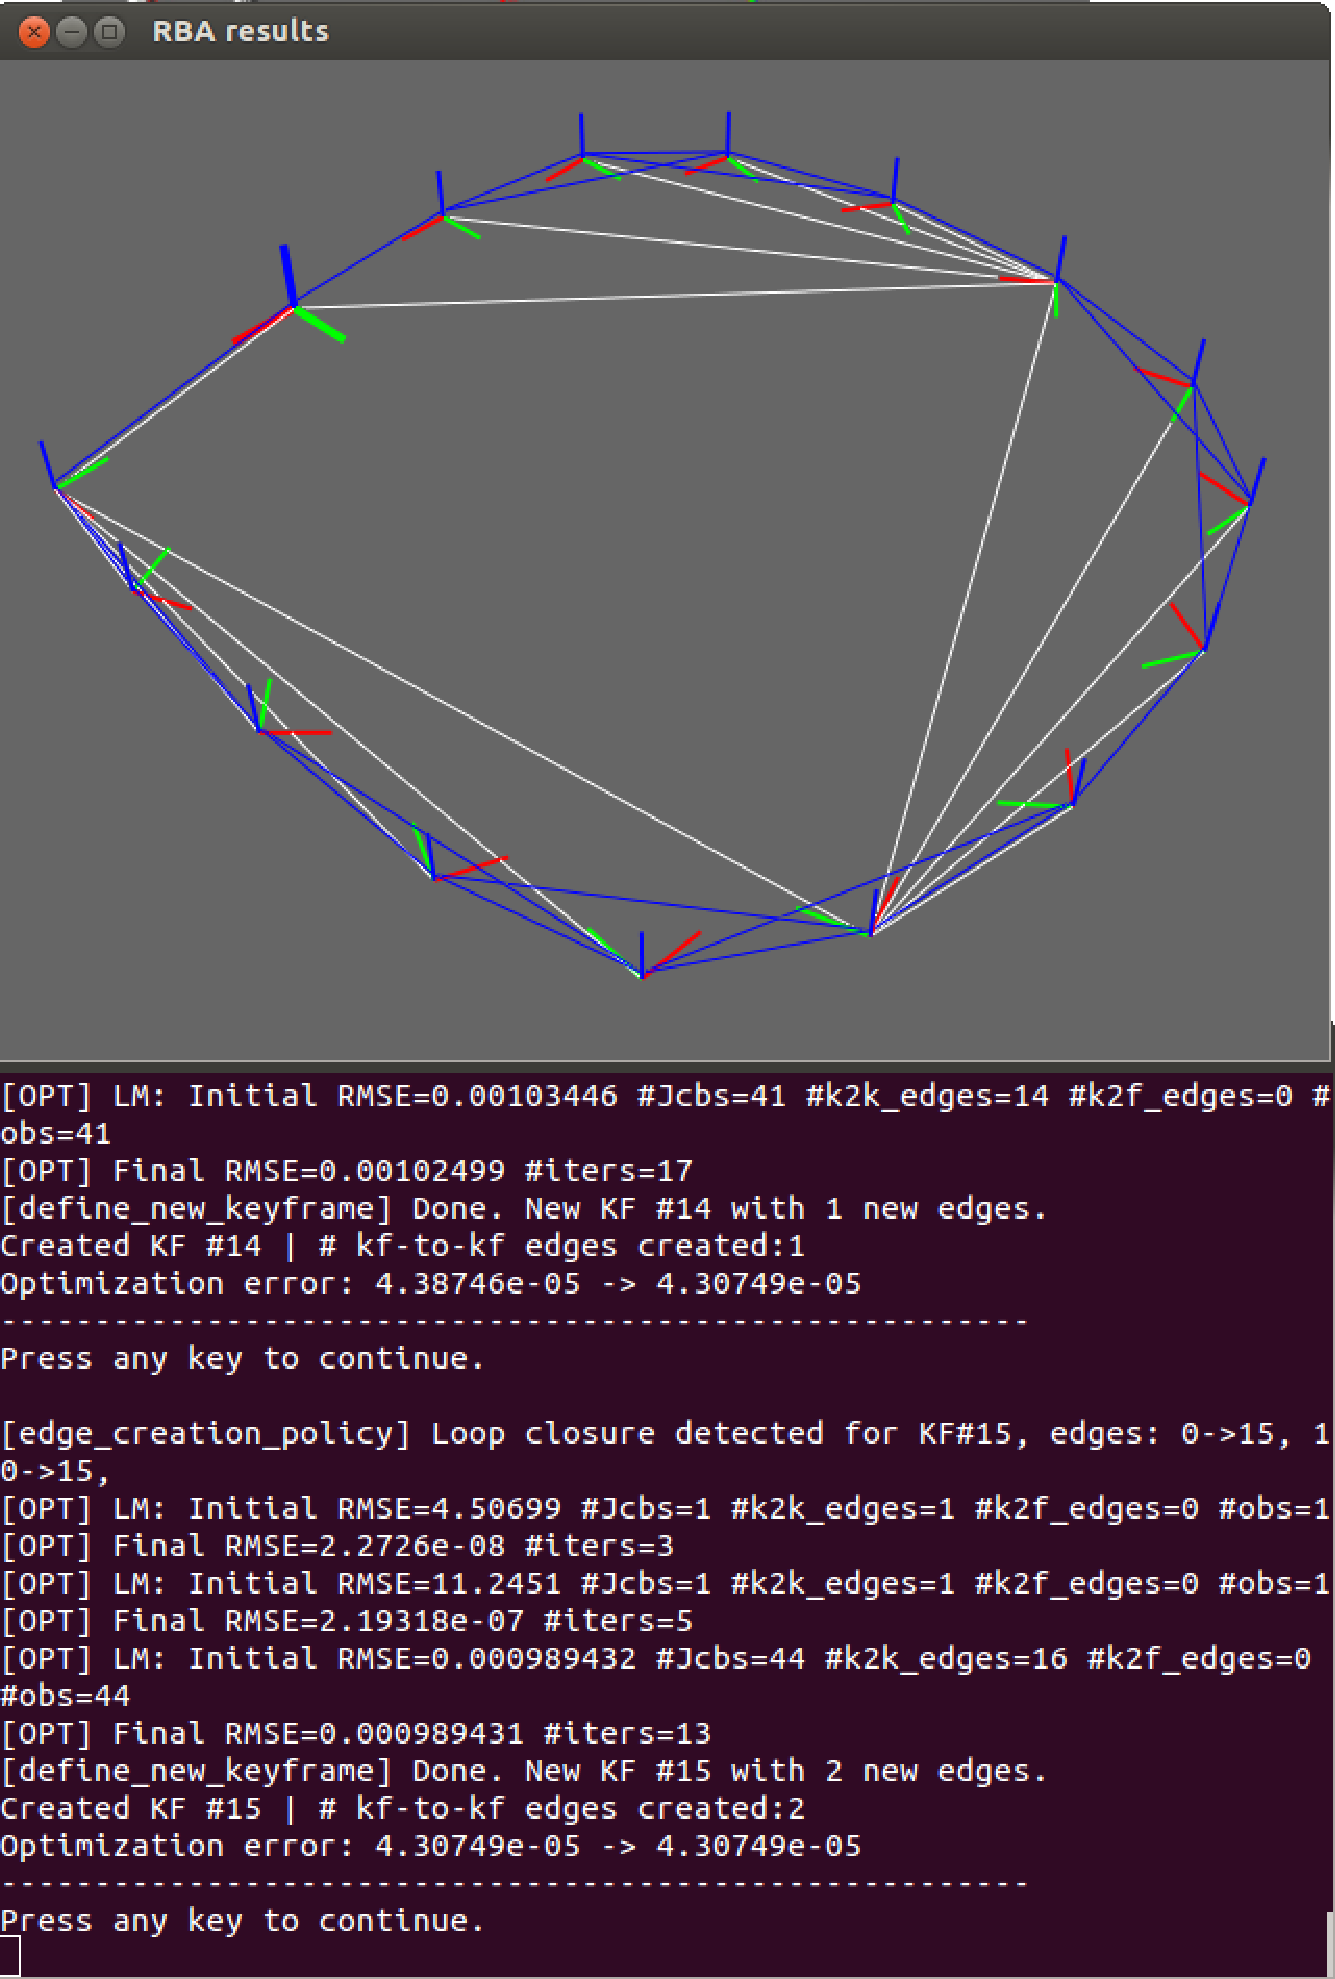
\includegraphics[width=0.8\textwidth]{imgs/screenshot_tutorial_relative-graph-slam-2D.pdf} 
\caption{Screenshot for \texttt{tutorial-srba-relative-graph-slam.cpp}.}
\label{fig:screenshot.tutorial2}
\end{figure}

\newpage

\section{Configuring \texttt{RbaEngine<>}: template arguments}
\label{sect:rba_configs}

In the following, all class names assume the existence of a previous:

\begin{lstlisting}
 using namespace mrpt::srba;
\end{lstlisting}



\subsection{\texttt{KF2KF\_POSE\_TYPE}: KF-to-KF relative poses}
\label{sec:k2k_types}

This template argument selects the model for the relative poses between keyframes. 
The two natural possibilities are SE(2) and SE(3) poses, which you should employ 
depending on whether your problem can be considered \emph{planar} or not:

\begin{itemize}
\item{\textbf{ \texttt{kf2kf\_poses::SE2} }: For 2D relative poses, i.e. they consists of a $(x,y)$ displacement 
plus a heading $\phi$. Poses are mapped to 
\href{http://reference.mrpt.org/stable/classmrpt_1_1poses_1_1_c_pose2_d.html}
{\texttt{mrpt::poses::CPose2D}} classes. 
}
\item{\textbf{ \texttt{kf2kf\_poses::SE3} }: For 3D relative poses. Given that the least-squares optimization runs 
on the linearized neighborhood of the manifold \cite{blanco2010tutorial} around the instantaneous solutions, the 
choice between different parameterizations (i.e. quaternions, Euler angles,etc.) becomes irrelevant. 
In this case poses become 
\href{http://reference.mrpt.org/stable/classmrpt_1_1poses_1_1_c_pose3_d.html}
{\texttt{mrpt::poses::CPose3D}}
classes, which internally hold the $3 \times 3$ rotation matrix for the SO(3) rotation and a $(x,y,z)$ vector 
for the translational part, with optional conversion to/from quaternions and yaw/pitch/roll angles.
}
\end{itemize}

Notice that the usage of 2D relative poses limits the robot trajectory to one single plane, but 
it does not mean that landmarks must also be 2D. It is perfectly legal to use planar poses with 3D landmarks.


\subsection{\texttt{LM\_TYPE}: Relative landmark parameterizations}
\label{sec:k2f_types}

XXXX XXXX 

\subsection{\texttt{OBS\_TYPE}: Observation types}

XXXX XXXX 


\subsection{Sensor models}
\label{sect:program_sensors}

XXXX XXXX 


\subsection{\texttt{RBA\_OPTIONS}: Other options}
\label{sect:rba_options}

XXXX XXXX 


\subsubsection{\texttt{sensor\_pose\_on\_robot\_t}}


\subsubsection{\texttt{obs\_noise\_matrix\_t}}


\subsubsection{\texttt{solver\_t}}


\section{Configuring \texttt{RbaEngine<>}: dynamic parameters}
\label{sect:rba_dyn_parameters}

Can be changed at run-time, not at build-time.

\subsection{Edge-creation policy}
\label{sect:edge.policy}

(...)

\subsection{Levenberg-Marquardt solver parameters}
\label{sect:lm-params}

(...)



\section{The \texttt{srba-slam} application}
\label{sect:srba_slam_app}

XXXX

\section{Library inner structure}

\subsection{Directory layout}


\subsection{Data structures}

\begin{sidewaysfigure}
\centering
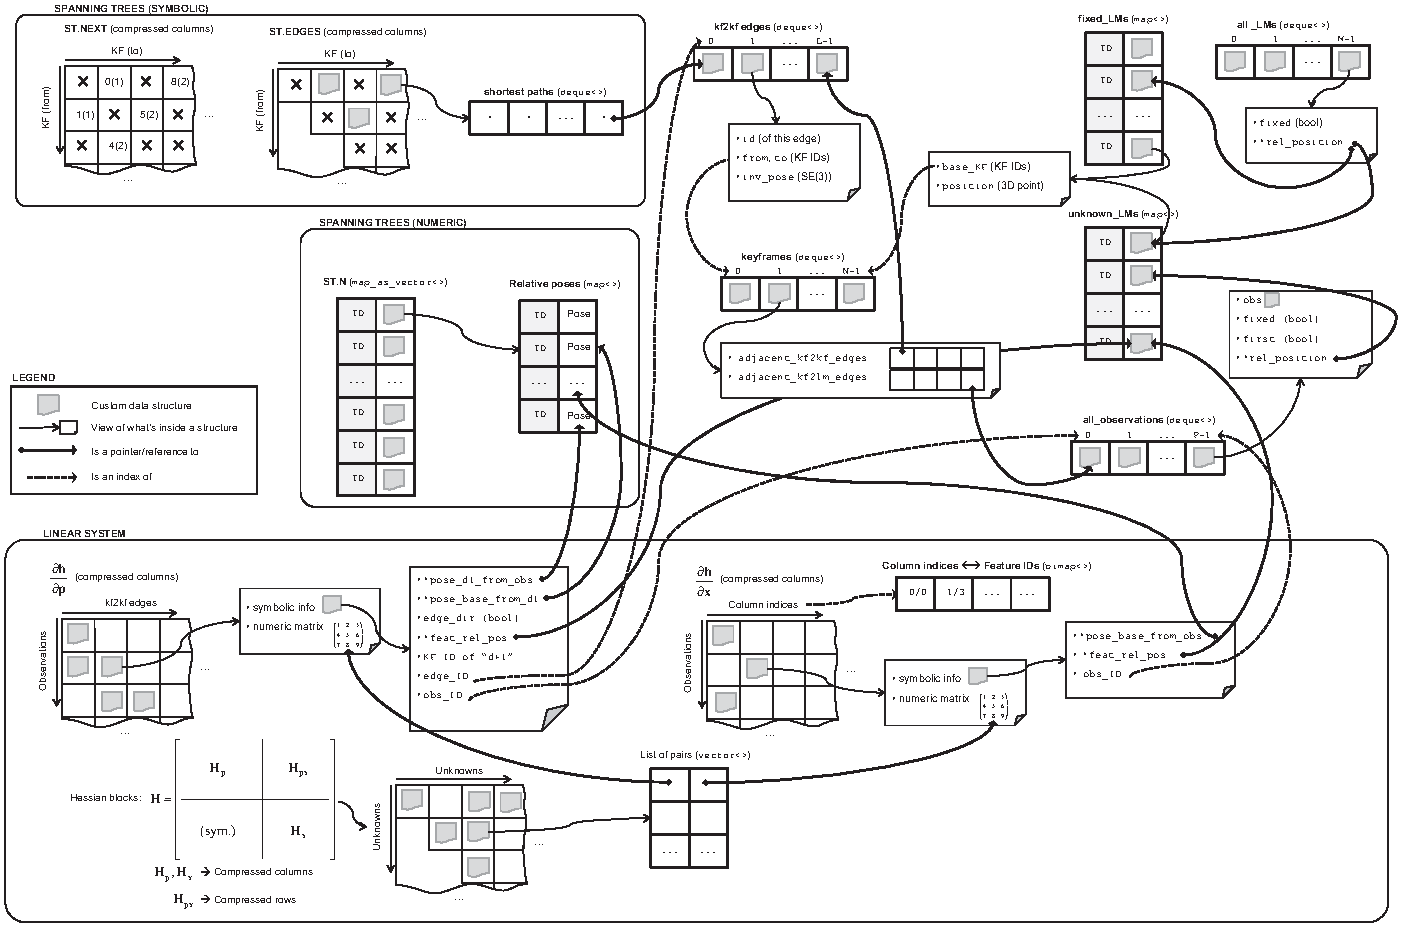
\includegraphics[width=1.0\textwidth]{imgs/srba_data_structures.pdf} 
\caption{Detailed data structures. Refer to the legend for the format of structures and pointers/references.}
\label{fig:detailed.data.structures}
\end{sidewaysfigure}



\newpage
\section{Pseudo-code}

The following symbols are employed in the following:

\begin{itemize}
\item{$D_{max}$: Maximum depth for which spanning trees are maintained. It is also the maximum topological distance 
   from the given KF to look for unknowns to optimize during a ``local area'' optimization. Obviously, all KFs within 
   that distance are also in the spanning tree.}
\item{$N_o$: Number of observed landmarks from the new KF being inserted in the problem.}
\item{$N_R$: The maximum number of reachable KFs for a fixed $D_{max}$. It is reasonable to consider that this number 
is bounded for any map, as long as redundant KFs are not continuously added for the same area.}
\item{$\gamma$: A constant coefficient that models the ``sparseness'' of the graph being solved by least-squares minimization.}
\item{$(\mathbf{z}_n^i,\mathbf{\alpha}_n^i)$: The $i-th$ individual observation of the $n-th$ time step, and 
  its corresponding data association (i.e. its correspondence, the ID of an existing landmark or a new ID if this 
  is a new LM).}
\end{itemize}


\newpage
\subsection{\texttt{define\_new\_keyframe()}}
\label{sect:code:define_new_keyframe}

%% ==============================================
%%  Alg: define_new_keyframe
%% ==============================================
%% ==============================================
%%  Alg: srba_process_new_kf
%% ==============================================
\begin{algorithm}
\BeginAlgSize
\caption{\texttt{srba\_define\_new\_keyframe}   \hfill 
 \textcolor{white}{.}
$\text{Worst case: }\Or( (\gamma N_R)^3+ N_o ( D_{max} + \log N_R)  )$  }
\label{alg:srba}
\begin{algorithmic}[1]
\Statex{C++: \texttt{RBA\_Problem::define\_new\_keyframe()}}
\Statex
  %\medskip
\Require{ $\left( \mathbf{z}_n,\mathbf{\alpha}_n \right) =
\left\{ \left( \mathbf{z}^1_n,\A^1_n \right),...,
   \left( \mathbf{z}^{N_o}_n,\A^{N_o}_n \right) \right\}$ 
\Comment{Set of $N_o$ new observations 
$\mathbf{z}^i_n$ and their data association $\A^i_n$ }}
\Require{ $run\_local\_optimization$ \Comment{Whether to also run optimizations}}
\Ensure { The updated, locally consistent map }
\Statex
%-----------
\Statex{\underline{// Update keyframes (KFs) data structures}}
\State{$n \gets $number of KFs in the map} \Comment{Assign a free ID to the new KF -- $\Or(1)$}
\State{$KF[n] \gets $empty KF data structure} \Comment{Insert at the end of \texttt{std::map} --
$\Or(1)$}
%-----------
\Statex
\Statex{\underline{// Apply edge-creation policy to decide how to handle loop closures, etc.}}
%% \State{$\mathbf{new\_edges} = \varnothing $}
\While{$ \varnothing \neq \left[ (i_k \leftrightarrow n) = \text{\texttt{decide\_edge\_to\_create}()}\right]$ }
  \Comment{\begin{tiny}$\Or(N_o \log N_R)$\end{tiny}}
	\State{\texttt{add\_kf2kf\_edge}$( i_k \leftrightarrow n )$ } 
	\Comment{Update KF-to-KF edge structures -- $\Or(1)$ }
\State{\texttt{update\_sym\_spanning\_trees}$( i_k \leftrightarrow n )$ }
\Comment{$\Or(N_R^2\log N_R)$}
\EndWhile \Comment{Typ. iterations: $\Or(\gamma)$}

%% ---
%-----------
\Statex
\Statex{\underline{// Update symbolic Jacobian structures}}
 \Comment{$\Or\left(N_o (D_{max}+ \log N_R) \right)$}
\ForEach{$ \left( \mathbf{z}_n^i,\mathbf{\alpha}_n^i \right) \in \left(
\mathbf{z}_n,\mathbf{\alpha}_n \right)$}  
\Comment{For each of the $N_o$ new observations}
	\State{\texttt{add\_observation}$(
 \underbrace{\mathbf{z}_n^i}_{\text{obs. data}},
 \underbrace{n}_{\text{observing KF}},
 \underbrace{\mathbf{\alpha}_n^i}_{\text{\text{landmark ID}}} 
)$ }
\Comment{\begin{tiny}$\Or(D_{max}+ \log N_R)$\end{tiny}}
\EndFor
%-----------
\Statex
\If{$run\_local\_optimization$}
\If{$optimize\_new\_edges\_alone$}
\Statex{~~~~~~~~\underline{// Initialize new edges}}
\ForEach{$ (i_k \leftrightarrow n) $} \Comment{For each new kf2kf edge created above}
\State{\texttt{non\_linear\_optimizer}$\left( i_k \leftrightarrow n \right)$} \Comment{$\Or(N_o)$}
\EndFor
\EndIf
%-----------
\Statex
\Statex{~~~~\underline{// Update SLAM estimation}}
\State{$\mathbf{edges\_to\_optimize} \gets$ all within a $D_{max}$ distance from $n$}
\Comment{$\Or(N_R)$}
\State{\texttt{non\_linear\_optimizer}$\left( \mathbf{edges\_to\_optimize}
\right)$} \Comment{$\Or( (\gamma N_R)^3)$}
\EndIf
\end{algorithmic}
\EndAlgSize
\end{algorithm}




\newpage
\subsection{\texttt{update\_sym\_spanning\_trees()}}

This algorithm is explained in \cite{blanco2013srba}.

%% ==============================================
%%  Alg: update_sp_sym
%% ==============================================
%% ==============================================
%%  Alg: update_sp_sym
%% ==============================================
\begin{algorithm}
\BeginAlgSize
\caption{\texttt{update\_sym\_spanning\_trees} \hfill 
 \textcolor{white}{.}
$\text{Worst case: }\Or(N_R^2 \log N_R)$ }
\label{alg:update_sp_sym}
\begin{algorithmic}[1]
  %\medskip
\Require{~\newline 
$(i_k \leftrightarrow n) $ \Comment{A new edge} }\newline
$D_{max}$ \Comment{The maximum desired depth of span. trees}
\Statex
%-----------
  \State{$ST_{D_{max}-1}(i_k) \gets \{ \forall v / d(v,i_k)\leq D_{max}-1 \}$}
    \Comment{$\Or(N_R)$}
  \State{$ST_{D_{max}}(n) \gets \{ \forall v / d(v,n)\leq D_{max} \}$}
    \Comment{$\Or(N_R)$}
   %\Comment{Changes with each $i_k$}
  \Statex
  \ForEach{$r \in ST_{D_{max}}(n)$} \Comment{$\Or(N_R)$ iterations}
   \ForEach{$s \in ST_{D_{max}-1}(i_k)$} \Comment{$\Or(N_R)$ iterations}
    \State{// New tentative distance between $r$ and $s$}
    \State{$d \gets \mathcal{ST.D}[n][r] + \mathcal{ST.D}[i_k][s] + 1 $}
      \Comment{$\Or(\log N_R)$}
     %\Comment{$\Or(\log X)$}
    \If{$\left(s \in \text{\texttt{spanning\_tree}}(r) \text{ \textbf{and} } d < \mathcal{ST.D}[r][s]\right)$ 
$\text{ \textbf{or} }$ $\left(s \notin \text{\texttt{spanning\_tree}}(r) \text{ \textbf{and} } d \leq D_{max}\right)$}
     \Comment{$\Or(\log N_R)$}
       \State{// Shorter or new path found. Update trees:}
       \State{$\mathcal{ST.D}[r][s] \gets d$}
       \State{$\mathcal{ST.N}[r][s] \gets \left\{
	\begin{array}{ll}
	  i_k  & r =n \\
	  \mathcal{ST.N}[r][n] & r \neq n 
	\end{array}
	\right. $}
       \State{$\mathcal{ST.D}[s][r] \gets d$}
        \Comment{$\Or(\log N_R)$}
       \State{$\mathcal{ST.N}[s][r] \gets \left\{
	\begin{array}{ll}
	  n  & s = i_k \\
	  \mathcal{ST.N}[s][i_k] & s\neq i_k 
	\end{array}
	\right. $}
    \EndIf
   \EndFor
  \EndFor
\end{algorithmic}
\EndAlgSize
\end{algorithm}
%% ==============================================






%% ---------------------------------------------------------------
%%                         BIBLIOGRAPHY
%% ---------------------------------------------------------------
\newpage
\bibliographystyle{plain}
\bibliography{cites}

\end{document}

